\newpage
\section{Group Evaluation}

We believe that the project was a productive exercise; our chosen team structure was very effective, and all team members made a significant and unique contribution. In this section, we evaluate the overall performance of our group and the processes we followed. We also discuss how we would improve our processes if we were to undertake a similar project in the future.

\subsection{Team Structure and Logistical Roles}
In our initial report (§6), we defined a team structure in which members adopted a logistical role in addition to any writing or programming responsibilities. There were several reasons why we decided to implement this structure:
\begin{itemize}[noitemsep]
	\item to ensure that administrative workload was divided evenly;
	\item to reduce the likelihood of conflicts or duplication of effort, by making it clear from the outset who is ultimately responsible for each area;
	\item to allow us to hold individuals to account in the unlikely event that work was not being completed in a timely fashion;
	\item to give everybody the opportunity to gain experience in management, report writing, and programming.
\end{itemize}

On balance, we believe this approach was highly effective -- team members quickly became familiar with their assigned roles. Arguably, the most difficult part was deciding what roles were necessary and allocating them in a way to fit people’s existing skillsets. It was also challenging to arbitrate effectively in the event that two or more people wanted to take on the same logistical role. We found that having some degree of flexibility with role titles and responsibilities helped us to arrive at our final role assignments.

Our fixed structure, however, did not come without problems. There were several occasions where team members were unavailable or away, rendering them unable to make important decisions. This left other team members wondering whether they should delay or proceed without the approval of the absent team member. In most cases, a delay could not be justified. It was clear that our contingency plans were insufficient, and in future we would make additional effort to ensure that a suitable backup plan was in place so that decisions could be taken in the absence of critical team members.

\subsection{Meetings and Communication}
\label{sec:meetings}
The team held meetings at least once every two days to discuss progress and assign work. Where possible, the Chair planned all meetings in advance, and compiled a formal agenda. The Secretary booked a meeting room to reduce distractions and ensure we had whiteboard facilities available. The Secretary also took minutes, which served as an important register of all the decisions we had taken in meetings. We made sure everybody was aware of upcoming meetings by using a shared calendar, and we enabled automated reminders in our group communication tool, Slack. Generally speaking, attendance at meetings was high. Latecomers sometimes caused delays, but the situation improved after we voiced our concerns. 

Particularly towards the end of the project, we found that meetings were called with short notice, and it therefore became difficult to create agendas in advance. We believe, in hindsight, that the team could have benefitted from a more fixed meeting schedule. That being said, many team members appreciated the flexibility to “work from home” in the later stages of the project, since they found that they were more productive when working alone. For this reason, we are unsure to what extent a more rigid meeting schedule would have actually improved our productivity.

\subsection{Planning and Scheduling}
The Chair and Secretary worked together to carefully plan out each phase of the project. We are very pleased that the team managed to adhere to this schedule closely. We had different phases for initial report writing, planning, implementation, final report writing, and presentation planning. These phases are presented graphically in the Gantt chart in Figure \ref{fig:gantt_chart}.

\begin{figure}[h!]
	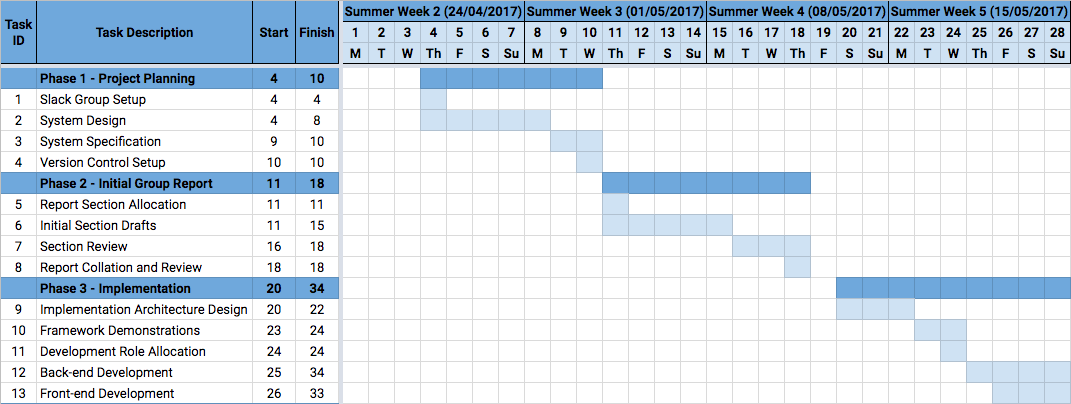
\includegraphics[width=\textwidth]{images/gantt_chart1}
	\vspace{0.1cm}\newline
	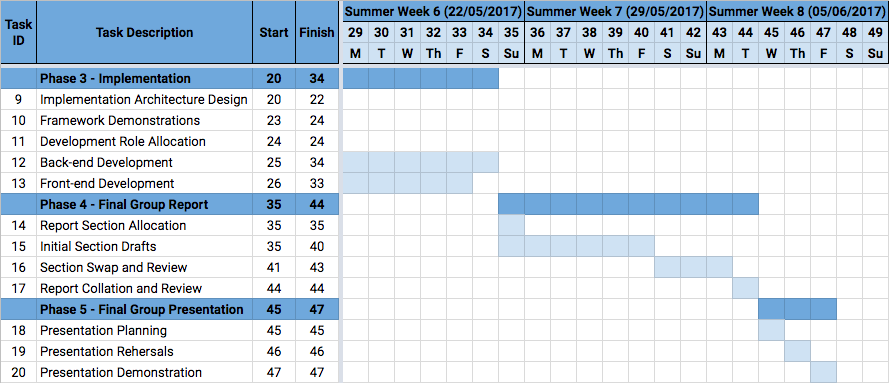
\includegraphics[width=0.83\textwidth]{images/gantt_chart2}
	\caption{Screenshots of the Gantt chart, showing the different phases throughout the project.}
	\label{fig:gantt_chart}
\end{figure}

\subsection{Writing and Documentation}
It appeared that some teams elected at an early stage to segregate their members into engineers and writers. We chose not to adopt the same approach for several reasons:

all members of the team were keen to get involved with programming tasks, and it would not have been reasonable to deprive them of this opportunity;
we collectively believed that the best person to write documentation for specific system components is the person who also wrote the code;
it would have been very challenging, and possibly wasteful, to write report sections as our solution was undergoing constant changes and adaptation.

Instead, our writing phase followed our implementation phase. We believe that this decision worked in our favour: since our prototype had been completed before writing started, we had little difficulty explaining how it worked. It was the first time many team members had to coordinate and delegate the writing of such a large report to so many people. 

We learned a lot from the process of writing the initial report, where we had not left sufficient time to proof-read, edit, and merge disparate report sections. For our final report, we adopted a three-stage review process to prevent a verbatim repeat of the difficulties we faced with our initial report. For both reports, it was sometimes challenging to assign writing tasks to relevant individuals whilst ensuring that the workload was evenly distributed.

\subsection{Daily Stand Ups}
\label{sec:standups}
We tracked the progress of individual team members and collected metrics through an automated daily stand-up process. While we had some initial reservations that people would forget to complete it, the participation rate was around 95\%. This gave us a comprehensive picture of our productivity and team sentiment. On several occasions, team members recorded low sentiment scores. We were able to investigate why people were unhappy, and address these problems as soon as they occurred. Since this process was fully automated, it required no additional effort from team members to coordinate. 

\begin{figure}[h!]
	\centering
	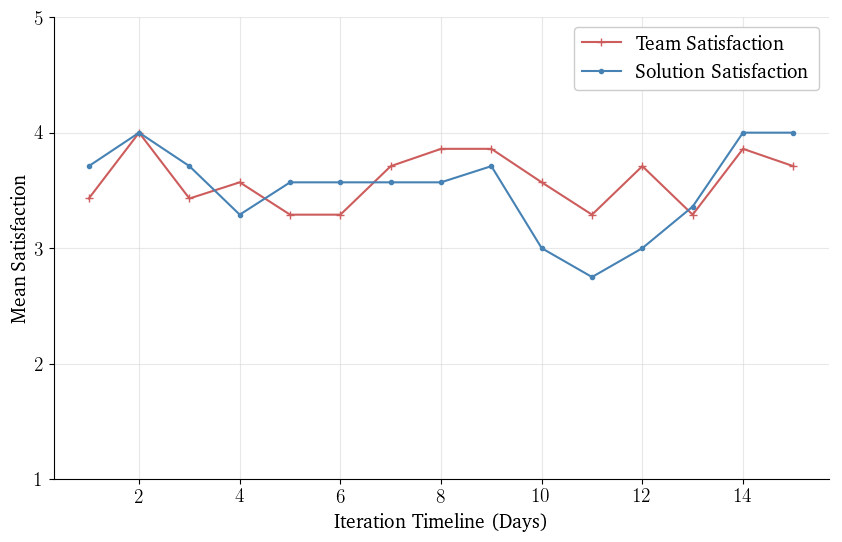
\includegraphics[width=0.8\textwidth]{images/plot_satisfaction}
	\caption{Mean satisfaction of team members with both the rest of the team, and the project solution.}
	\label{fig:plot_satisfaction}
\end{figure}

The burndown chart in Figure \ref{fig:plot_story_points} illustrates some of the metrics we were able to collect during the daily stand up. Amongst other things, we recorded the number of story points that each team member completed per day. 

\begin{figure}[h!]
	\centering
	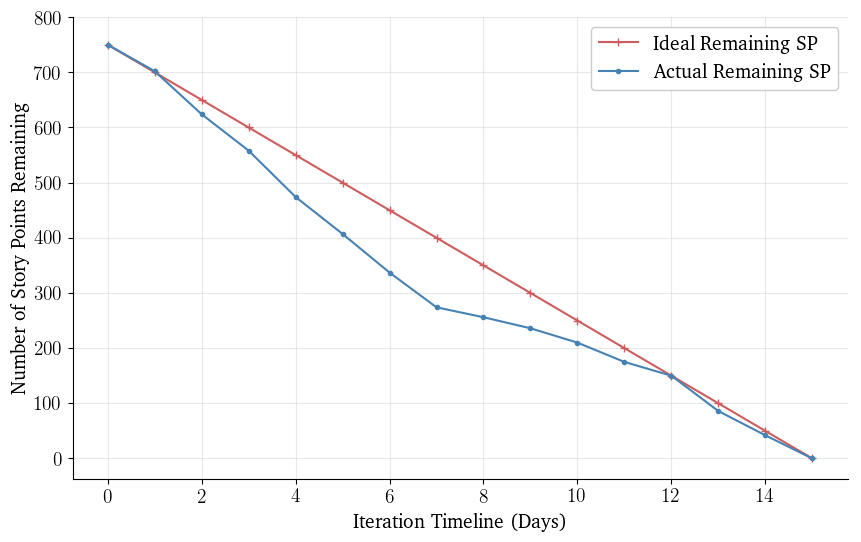
\includegraphics[width=0.8\textwidth]{images/plot_story_points}
	\caption{Burndown chart showing the actual rate of story point completion compared to the ideal rate.}
	\label{fig:plot_story_points}
\end{figure}

We also included in the daily stand up a range of qualitative open-answer questions, such as “What progress do you hope to complete before the next stand up?” and “What obstacles do you anticipate facing?”. These facilitated reflection, but were sometimes seen as burdensome, and we would probably include less of these questions if we were to undertake a similar project in future. We found that, while they improved the ability of the team to focus, they did not tell us anything we didn’t already know.

\subsection{Issue Tracking and Code Maturity}
\label{sec:issuetracking}
We used GitHub Issues to record pending tasks and faults identified with our code. We then placed these issues on a `kanban board’, allowing us to keep track of the current status of each ticket. A screenshot of our kanban board is provided in Figure \ref{fig:kanban_board}.

\begin{figure}[h!]
	%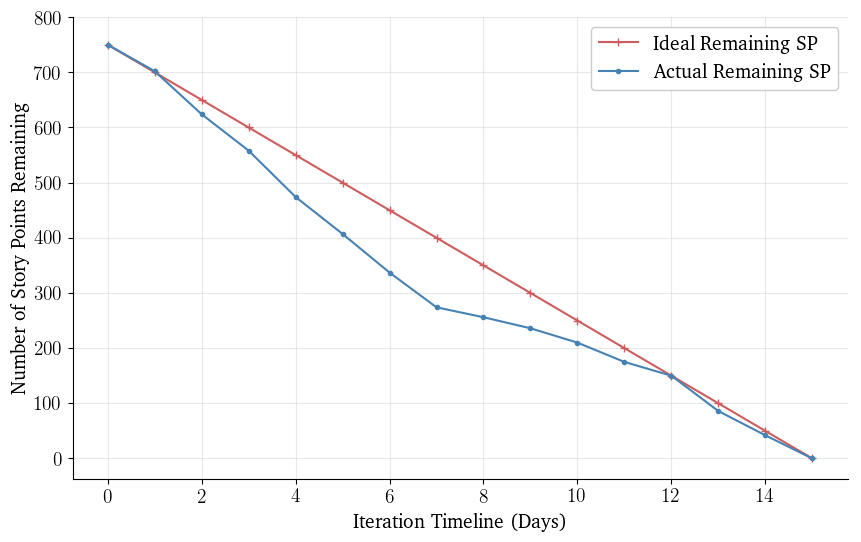
\includegraphics[width=\textwidth]{images/plot_story_points}
	\caption{Example of the kanban board during development.}
	\label{fig:kanban_board}
\end{figure}

\begin{figure}[h!]
	\centering
	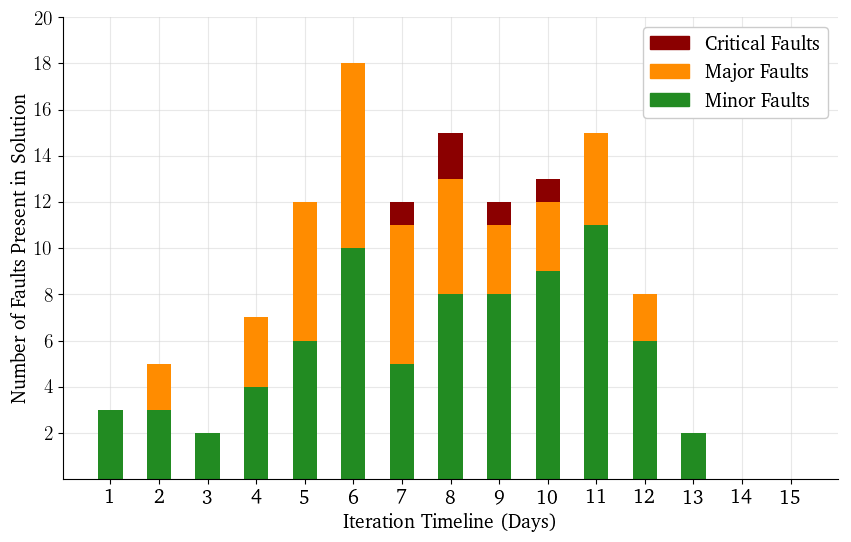
\includegraphics[width=0.8\textwidth]{images/plot_faults}
	\caption{Number of critical, major and minor faults present in the solution.}
	\label{fig:plot_faults}
\end{figure}



We used issue tickets to triage issues and assign a number of story points to each, indicating the amount of development effort that the issue ticket would require to complete. We found that this provided useful reference information when completing the daily stand up. However, we sometimes forgot to create or update issue tickets, meaning that the kanban board was not always up to date. In future, we would make more of an effort to create all of our tickets at the start of each agile sprint, along with story point estimations. We would also schedule a short daily review session to make sure that completed issues are always marked as resolved.


\subsection{Architecture Selection and Programming}
All team members took part in programming activities, allowing us to draw upon a very broad range of experience. Deciding on programming languages and frameworks was not a straightforward task, and we had to reconcile several opposing viewpoints. We were able to reach a consensus through compromise: splitting our code base into `front-end’ and`back-end’ components, each using a different language and set of frameworks. Those who were initially less comfortable with one of the languages were able to learn from those who were. Incidentally, this structure worked strongly in our favour, and we believe our solution was far superior to any we could have produced using just a single language.

We followed agile practices, allowing us to iterate quickly, mitigate risks, and come up with a `minimum viable product’ as early as possible. We felt that this was the most appropriate strategy given the tight time scale. By design, agile involves less onerous and detailed planning -- which we found to be both a blessing and a curse. We firmly believe that it would have been impossible to plan out all of our development efforts right at the beginning, and agile afforded us the capability of planning as we went along. However, there were several scenarios in which well-intentioned team members devoted a lot of effort to completing their tasks only to discover that their code was not fully compatible with what others had developed. This resulted in tedious merge conflicts that could have been avoided with more meticulous planning.

\subsection{Risk Management}
In the initial report (§10), we included a register of the main risks involved with our project.  We found that risks did not need to be added or removed as development progressed. Thankfully, many of the risks in the register (R2, R3, R5, R7, R9, R10) did not materialise because we took adequate reduction measures. However, other risks did materialise in some form. 
\begin{description}
	\item[R1: Unavailability of Team Members] There were several occasions where team members were ill or had other work to complete, meaning that tasks took them longer to complete than anticipated. We were able to mitigate this risk by building resilience into our schedule, ensuring disruptions did not significantly impact progress. In hindsight, we believe that we underestimated the likelihood of this risk occurring, but also overestimated the impact. We were able to work around disruptions effectively, meaning that an impact value of `high’ was not warranted.
	\item[R4: Incompatibilities and Merge Conflcits] We were often delayed due to code incompatibilities and merge conflicts. We believe that our assigned values for likelihood and impact were appropriate, because the occurrence of this risk did have a substantial impact. Simply communicating ownership did not turn out to be a sufficient reduction measure. In future, we would also ensure that distinct logical system components have a formal predefined common interface before programming begins.
	\item[R6: Collection of Metrics] As discussed in Section \ref{sec:standups}, we were able to gather most of our metrics through the daily stand ups, with a very high completion rate. However, not all story points were accounted for due to tickets not always being created. As we mentioned in Section \ref{sec:issuetracking}, we would employ additional measures in future to prevent this from happening. We believe that we overestimated the likelihood of this risk occurring, and in future we would assign a value of `medium’ instead. This is because our automated reminder system was very effective.
	\item[R8: Lateness to Meetings] Team members were sometimes unaware of what other members in the team were working on because of lateness or poor attendance to meetings. We acted quickly to raise concerns whenever necessary. We believe that our mitigation measures for this risk were appropriate. 
\end{description}
